\documentclass{article}
\usepackage[utf8]{inputenc}
\usepackage{enumitem}
\usepackage{xcolor}
\usepackage{graphicx}

\title{BooX}
\author{Huascar Retrieval Team}
\date{April 2020}

\begin{document}

\maketitle
\begin{center}
    
\includegraphics[scale=0.1]{img/logo.png}
\end{center}
\section{Problem}
\begin{itemize}[label={}]
    \item \textbf{Problem 1:} People who would like to get second-hand books at a lower price, fast, and without exposing themselves to dangerous places. 
    
    \item \textbf{Problem 2:} People who would like to save some space at home by getting rid of unused books, and potentially earning something in return.
    
\end{itemize}

\section{Objectives}
\begin{itemize}
    \item Encourage people to exchange their books, allowing them to read more books, increasing the read-culture in the country. 
    \item Connect people who want to get second-hand books and people who want to get rid of them. 
    \item Let the users sell/exchange their books in a reliable way.
\end{itemize}

\section{Target Market}
\begin{itemize}[label={}]
    \item \textbf{Target 1:} College students (17-25 y/o)\\
    They need educational books for their classes and some prefer physical books (no PDFs or eBooks) for the semester. Unfortunately, the books are usually very expensive \footnote{Ex.: Introduction to Algorithms by Thomas Cormen costs around \$100} and students can not afford them.
    \item \textbf{Target 2:} Youngsters and adults who enjoy reading (16-35 y/o)\\
    They prefer classic or young teenage novels. In both cases, unless the owner is a huge fan and rereads it occasionally, they are usually collecting dust in many households. Classics also tend to be expensive, and newer teenage novels are do not usually leave a good enough reason to read it again.
    
\end{itemize}

\section{Project Description}

Our project, called BooX, consists of a web app that facilitates the sale and interchange of used books by allowing users to upload their entire library with minimal effort, thus enabling our quick search system to put this huge database at the request of enthusiasts that are looking for that specific book they can not find or afford, or people who just want to put their library in the web and see if they get any offers. The main activities in this app would be the sale of books via mutual agreement between the owner and the buyer, and the exchange of books between owners. Whenever a sale or exchange is agreed, the participants must agree on a common place of exchange, where they have to meet physically to finalize the transaction.

Another important feature of the website is its automation capability, meaning any user who uploads his/her library can receive a notification (via email) when a user is interested on his/her book and, similarly, users who haven't uploaded their libraries will see a list of the top searched books or genres, giving them the possibility of matching an offer with one of their books.

As a whole, this project will fill a spot in the second-hand market, potentially improving the sales of valuable second-hand books by giving the owners a secure and fast to platform to generate revenue or exchange through these items.

\begin{center}
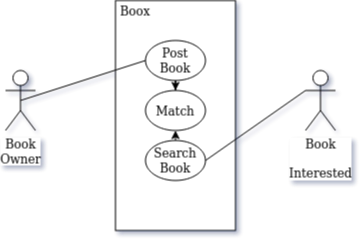
\includegraphics[scale=0.5]{img/diagram.png}    
\end{center}

\end{document}
